%% GENERATED by tools/from_docs.py from stepss-docs. Do not edit by hand:
%% edit the page named below in stepss-docs and regenerate.
%% source: stepss-docs/src/content/docs/test-systems/gb-network.md

\chapter{The Great Britain network}\label{doc:ts-gb}

The GB Network is a 50 Hz reduced-order representation of the Great Britain transmission grid with 87 buses and 37 synchronous machines (thermal and CCGT units with AVR/PSS and governor models), shunt compensation, and HVDC interconnections modelled as two-port converter injectors. It is used for dynamic simulation and wide-area monitoring/control studies; a one-line diagram is included in the repository.

\textbf{Repository:} \href{https://github.com/SPS-L/stepss-GB-Network}{SPS-L/stepss-GB-Network}

\section{One-line Diagram}\label{ts-gb:one-line-diagram}

\begin{figure}[htbp]
\centering
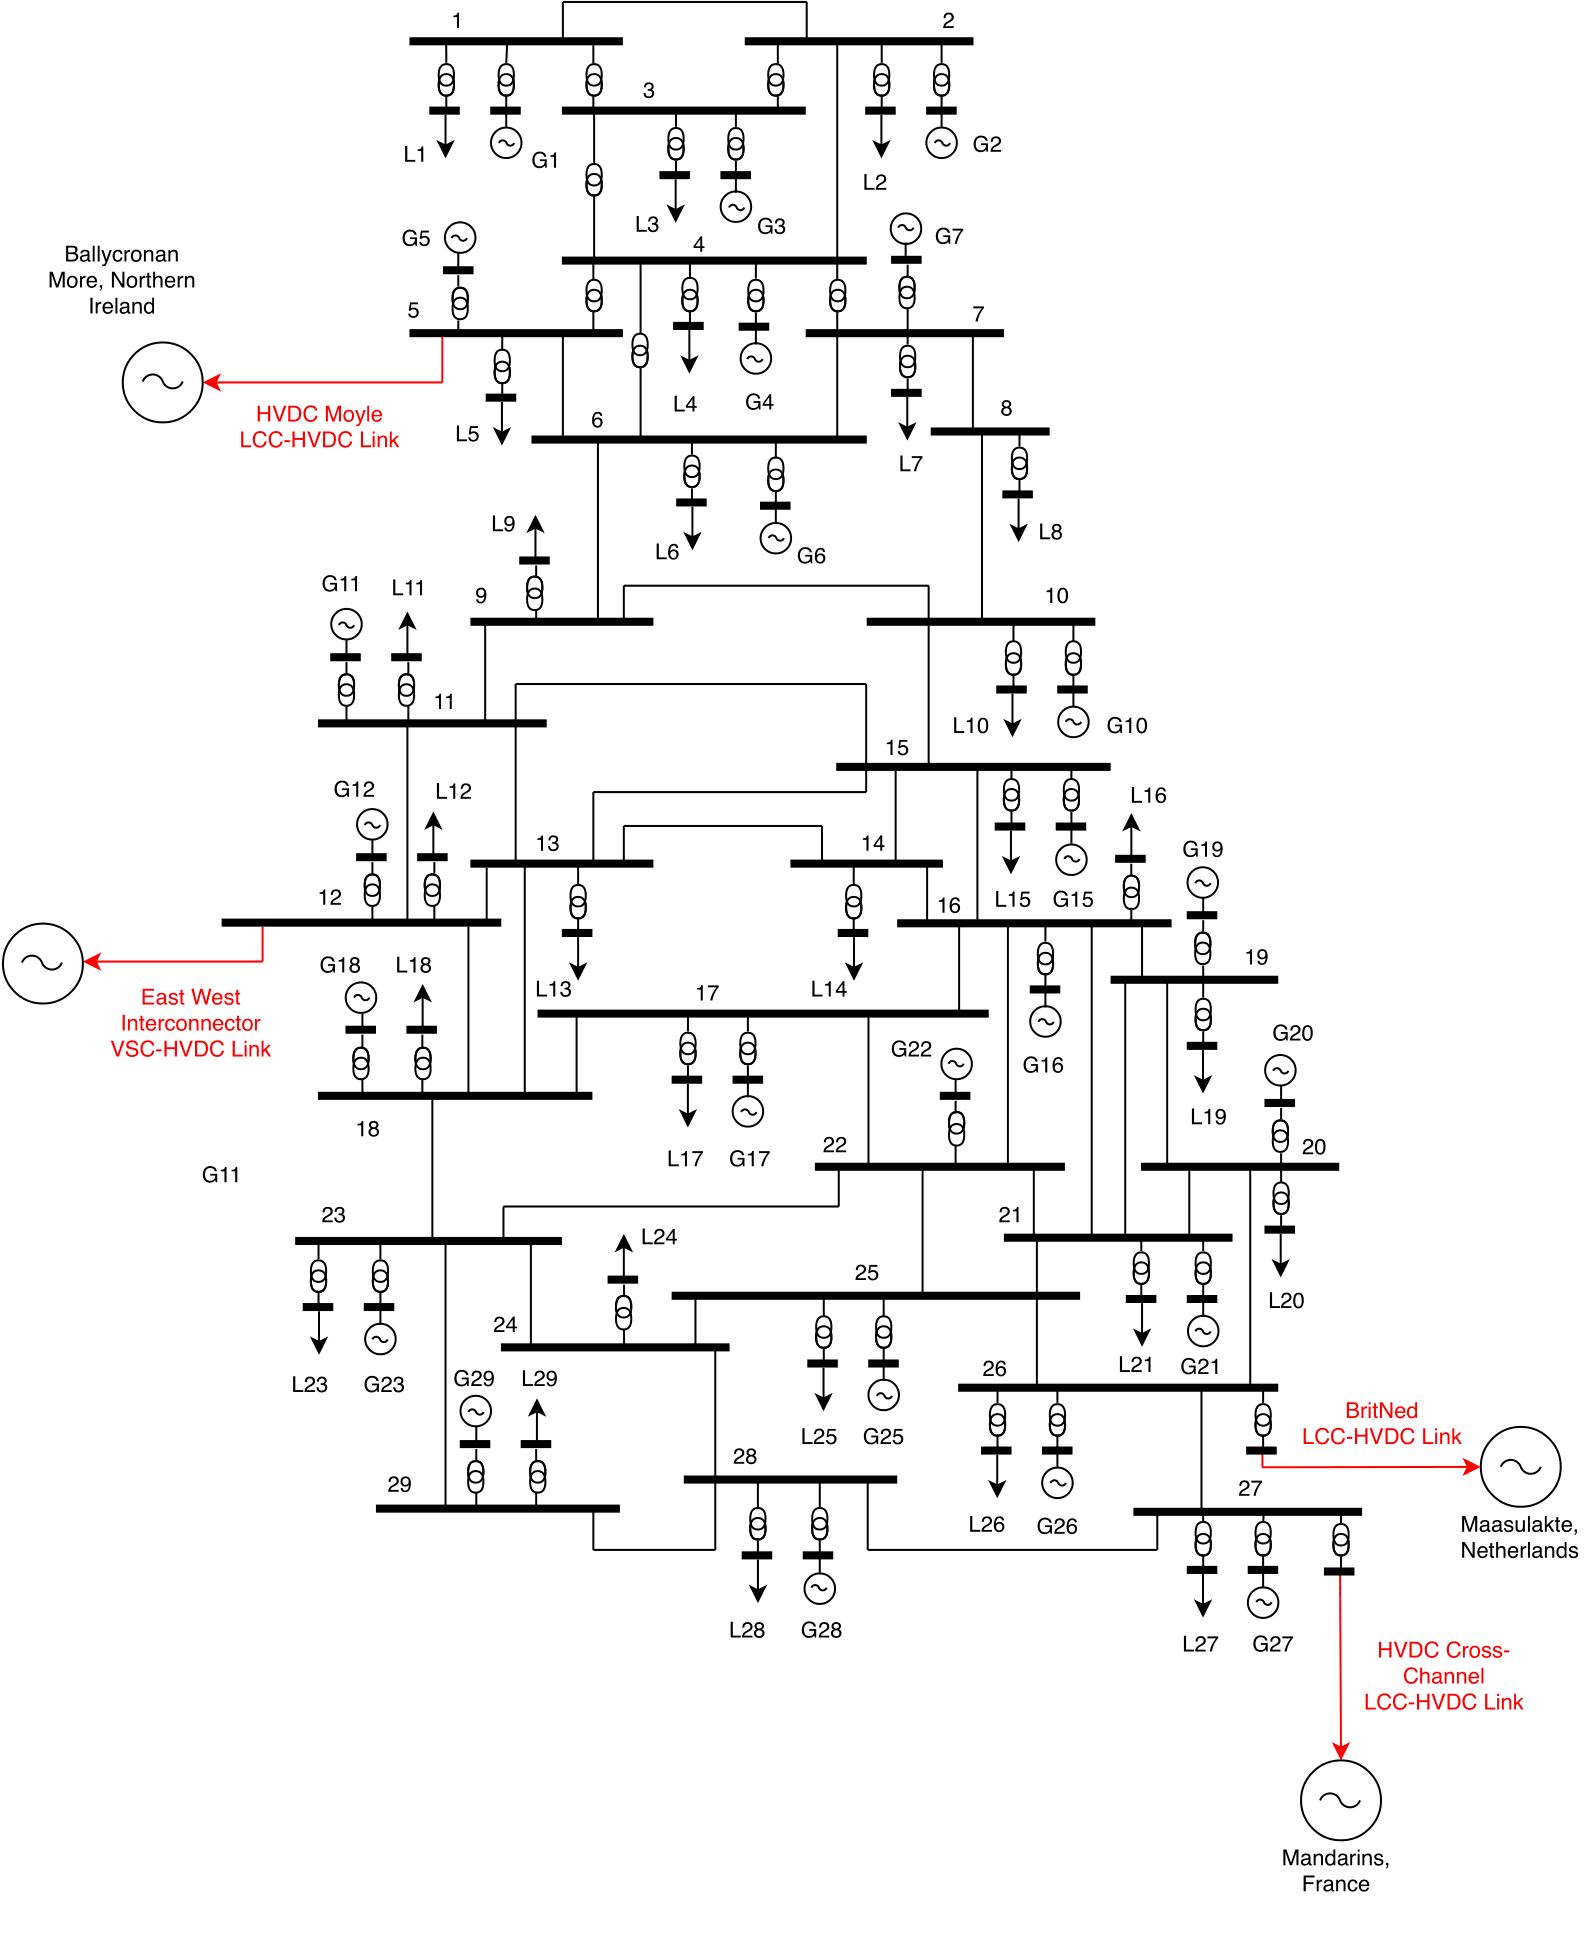
\includegraphics[width=0.80\linewidth]{figures/gb_oneline}
\caption{One-line diagram of the GB network with HVDC-LCC links}
\end{figure}

\begin{center}\rule{0.5\linewidth}{0.5pt}\end{center}

\section{Quick Start}\label{ts-gb:quick-start}

\begin{Verbatim}
import stepss

case = stepss.cfg()
case.addData('GBdyn.dat')      # dynamic data: machines, exciters/PSS, governors, loads
case.addData('GBhvdc.txt')     # HVDC interconnection two-port models
case.addData('GBvoltrat.dat')  # power-flow solution
case.addData('settings.dat')   # solver settings
case.addDst('disturb.dst')     # 180 s run with commented disturbance templates
case.addObs('obs.dat')         # observables to record

sim = stepss.sim()
sim.execSim(case)
\end{Verbatim}

The disturbance file contains ready-made (commented) templates for line and machine trips, bus faults, and HVDC parameter changes; uncomment and adapt them as needed. Alternatively, run the RAMSES executable directly with the included \texttt{cmd.txt}.

\begin{center}\rule{0.5\linewidth}{0.5pt}\end{center}

\section{Download}\label{ts-gb:download}

The test system files are available in the \href{https://github.com/SPS-L/stepss-GB-Network}{stepss-GB-Network repository}.

\section{See Also}\label{ts-gb:see-also}

\begin{itemize}
\tightlist
\item
  \hyperref[doc:ts-index]{Test Systems}, the other benchmark networks
\item
  \hyperref[doc:model-twop]{Two-Port Models}, the HVDC converter models used here
\item
  \hyperref[ch-disturb]{Disturbances}, syntax for the commented templates in \texttt{disturb.dst}
\end{itemize}
